\documentclass[10pt,conference]{IEEEtran}
\IEEEoverridecommandlockouts
\usepackage[T1]{fontenc}
\usepackage[utf8]{inputenc}
\usepackage{booktabs}
\usepackage{graphicx}
\usepackage{url}
\usepackage{xcolor}
\usepackage{microtype}
\usepackage[hidelinks]{hyperref}
\usepackage{balance}
\newcommand{\NSetups}{2,660}
\newcommand{\NCollections}{511}
\newcommand{\NCorpus}{3,171}
\newcommand{\NPinnedOk}{3,130}
\newcommand{\NHeadOk}{3,133}
\newcommand{\NPinnedUnfetchable}{36}
\newcommand{\NHeadUnfetchable}{33}
\newcommand{\NMovedHead}{1,694}
\newcommand{\PctMovedHead}{54.1}
\newcommand{\NGoneAfterPin}{0}
\newcommand{\NPinnedLintFailed}{5}
\newcommand{\SOneSetups}{293}
\newcommand{\SOneSetupsPct}{11.0}
\newcommand{\SOneCols}{1}
\newcommand{\SOneColsPct}{0.2}
\newcommand{\SOneOldSetups}{259}
\newcommand{\SOneOldSetupsPct}{9.7}
\newcommand{\STwoSetups}{63}
\newcommand{\STwoSetupsPct}{2.4}
\newcommand{\STwoCols}{0}
\newcommand{\STwoColsPct}{0.0}
\newcommand{\STwoOldSetups}{65}
\newcommand{\STwoOldSetupsPct}{2.4}
\newcommand{\SThreeSetups}{261}
\newcommand{\SThreeSetupsPct}{9.8}
\newcommand{\SThreeCols}{64}
\newcommand{\SThreeColsPct}{12.5}
\newcommand{\SThreeOldSetups}{101}
\newcommand{\SThreeOldSetupsPct}{3.8}
\newcommand{\QOneSetups}{20}
\newcommand{\QOneSetupsPct}{0.8}
\newcommand{\QOneCols}{0}
\newcommand{\QOneColsPct}{0.0}
\newcommand{\QOneOldSetups}{20}
\newcommand{\QOneOldSetupsPct}{0.8}
\newcommand{\POneSetups}{62}
\newcommand{\POneSetupsPct}{2.3}
\newcommand{\POneCols}{18}
\newcommand{\POneColsPct}{3.5}
\newcommand{\POneOldSetups}{60}
\newcommand{\POneOldSetupsPct}{2.3}
\newcommand{\PTwoSetups}{6}
\newcommand{\PTwoSetupsPct}{0.2}
\newcommand{\PTwoCols}{0}
\newcommand{\PTwoColsPct}{0.0}
\newcommand{\PTwoOldSetups}{4}
\newcommand{\PTwoOldSetupsPct}{0.2}
\newcommand{\PThreeSetups}{450}
\newcommand{\PThreeSetupsPct}{16.9}
\newcommand{\PThreeCols}{127}
\newcommand{\PThreeColsPct}{24.9}
\newcommand{\PThreeOldSetups}{73}
\newcommand{\PThreeOldSetupsPct}{2.7}
\newcommand{\AnySSetups}{574}
\newcommand{\AnySSetupsPct}{21.6}
\newcommand{\AnySCols}{65}
\newcommand{\AnySColsPct}{12.7}
\newcommand{\AnySOldSetups}{407}
\newcommand{\AnySOldSetupsPct}{15.3}
\newcommand{\AnyQSetups}{20}
\newcommand{\AnyQSetupsPct}{0.8}
\newcommand{\AnyQCols}{0}
\newcommand{\AnyQColsPct}{0.0}
\newcommand{\AnyQOldSetups}{20}
\newcommand{\AnyQOldSetupsPct}{0.8}
\newcommand{\AnyPSetups}{67}
\newcommand{\AnyPSetupsPct}{2.5}
\newcommand{\AnyPCols}{18}
\newcommand{\AnyPColsPct}{3.5}
\newcommand{\AnyPOldSetups}{63}
\newcommand{\AnyPOldSetupsPct}{2.4}
\newcommand{\AnySixSetups}{639}
\newcommand{\AnySixSetupsPct}{24.0}
\newcommand{\AnySixCols}{81}
\newcommand{\AnySixColsPct}{15.9}
\newcommand{\AnySixOldSetups}{471}
\newcommand{\AnySixOldSetupsPct}{17.7}
\newcommand{\AnySixPlusSetups}{880}
\newcommand{\AnySixPlusSetupsPct}{33.1}
\newcommand{\AnySixPlusCols}{175}
\newcommand{\AnySixPlusColsPct}{34.2}
\newcommand{\AnySixPlusOldSetups}{527}
\newcommand{\AnySixPlusOldSetupsPct}{19.8}
\newcommand{\CondSOneofmcp}{27.6}
\newcommand{\CondSTwoofhooks}{11.8}
\newcommand{\CondSThreeofskills}{13.1}
\newcommand{\CondQOneofagents}{2.6}
\newcommand{\DenSetupsWithMcp}{1,063}
\newcommand{\DenSetupsWithHooks}{533}
\newcommand{\DenSetupsWithSkills}{1,988}
\newcommand{\DenSetupsWithAgents}{773}
\newcommand{\DenCollectionsWithSkills}{511}
\newcommand{\LadderOldRawThirtyOne}{769}
\newcommand{\LadderOldRawSix}{602}
\newcommand{\LadderOldClass}{503}
\newcommand{\LadderOldNofind}{488}
\newcommand{\LadderOldFinal}{471}
\newcommand{\LadderOldRawThirtyOnePct}{28.9}
\newcommand{\LadderOldRawSixPct}{22.6}
\newcommand{\LadderOldClassPct}{18.9}
\newcommand{\LadderOldNofindPct}{18.3}
\newcommand{\LadderOldFinalPct}{17.7}
\newcommand{\LadderNewRawThirtyOne}{1064}
\newcommand{\LadderNewRawSix}{954}
\newcommand{\LadderNewClass}{656}
\newcommand{\LadderNewNofind}{656}
\newcommand{\LadderNewFinal}{639}
\newcommand{\LadderNewRawThirtyOnePct}{40.0}
\newcommand{\LadderNewRawSixPct}{35.9}
\newcommand{\LadderNewClassPct}{24.7}
\newcommand{\LadderNewNofindPct}{24.7}
\newcommand{\LadderNewFinalPct}{24.0}
\newcommand{\InstSOneOld}{256}
\newcommand{\InstSOneNew}{294}
\newcommand{\InstSOneLost}{0}
\newcommand{\InstSOneGained}{38}
\newcommand{\InstSTwoOld}{63}
\newcommand{\InstSTwoNew}{63}
\newcommand{\InstSTwoLost}{0}
\newcommand{\InstSTwoGained}{0}
\newcommand{\InstSThreeOld}{117}
\newcommand{\InstSThreeNew}{325}
\newcommand{\InstSThreeLost}{0}
\newcommand{\InstSThreeGained}{208}
\newcommand{\InstQOneOld}{20}
\newcommand{\InstQOneNew}{20}
\newcommand{\InstQOneLost}{0}
\newcommand{\InstQOneGained}{0}
\newcommand{\InstPOneOld}{77}
\newcommand{\InstPOneNew}{80}
\newcommand{\InstPOneLost}{0}
\newcommand{\InstPOneGained}{3}
\newcommand{\InstPTwoOld}{4}
\newcommand{\InstPTwoNew}{6}
\newcommand{\InstPTwoLost}{0}
\newcommand{\InstPTwoGained}{2}
\newcommand{\InstSOneGainTag}{18}
\newcommand{\InstSOneGainDiscovery}{2}
\newcommand{\InstSOneGainContainer}{2}
\newcommand{\InstSOneGainGit}{1}
\newcommand{\InstSOneGainOther}{15}
\newcommand{\InstSThreeGainString}{202}
\newcommand{\InstSThreeGainList}{0}
\newcommand{\InstSThreeGainMixed}{0}
\newcommand{\InstSThreeGainUnverified}{0}
\newcommand{\InstSThreeGainChecked}{202}
\newcommand{\PersSOneFlaggedAtPin}{294}
\newcommand{\PersSOneStillAtHead}{277}
\newcommand{\PersSOneResolvedAtHead}{17}
\newcommand{\PersSOneRepoGone}{0}
\newcommand{\PersSOneNewAtHead}{2}
\newcommand{\PersSOneResolvedPctOfRescanned}{5.8}
\newcommand{\PersSTwoFlaggedAtPin}{63}
\newcommand{\PersSTwoStillAtHead}{62}
\newcommand{\PersSTwoResolvedAtHead}{1}
\newcommand{\PersSTwoRepoGone}{0}
\newcommand{\PersSTwoNewAtHead}{0}
\newcommand{\PersSTwoResolvedPctOfRescanned}{1.6}
\newcommand{\PersSThreeFlaggedAtPin}{325}
\newcommand{\PersSThreeStillAtHead}{313}
\newcommand{\PersSThreeResolvedAtHead}{12}
\newcommand{\PersSThreeRepoGone}{0}
\newcommand{\PersSThreeNewAtHead}{3}
\newcommand{\PersSThreeResolvedPctOfRescanned}{3.7}
\newcommand{\PersQOneFlaggedAtPin}{20}
\newcommand{\PersQOneStillAtHead}{19}
\newcommand{\PersQOneResolvedAtHead}{1}
\newcommand{\PersQOneRepoGone}{0}
\newcommand{\PersQOneNewAtHead}{0}
\newcommand{\PersQOneResolvedPctOfRescanned}{5.0}
\newcommand{\PersPOneFlaggedAtPin}{80}
\newcommand{\PersPOneStillAtHead}{75}
\newcommand{\PersPOneResolvedAtHead}{5}
\newcommand{\PersPOneRepoGone}{0}
\newcommand{\PersPOneNewAtHead}{0}
\newcommand{\PersPOneResolvedPctOfRescanned}{6.2}
\newcommand{\PersPTwoFlaggedAtPin}{6}
\newcommand{\PersPTwoStillAtHead}{2}
\newcommand{\PersPTwoResolvedAtHead}{4}
\newcommand{\PersPTwoRepoGone}{0}
\newcommand{\PersPTwoNewAtHead}{0}
\newcommand{\PersPTwoResolvedPctOfRescanned}{66.7}
\newcommand{\DeclFiles}{2,593}
\newcommand{\DeclTotal}{3,923}
\newcommand{\DeclRemote}{1,488}
\newcommand{\DeclPackage}{1,476}
\newcommand{\DeclLocal}{954}
\newcommand{\DeclOther}{5}
\newcommand{\DeclPackagePinned}{157}
\newcommand{\DeclPackageUnpinned}{1,129}
\newcommand{\DeclPackageTag}{190}
\newcommand{\DeclPctUnpinnedOrTag}{89.4}
\newcommand{\DeclPctPackage}{37.6}
\newcommand{\DeclSetupsWithAny}{1053}
\newcommand{\AuditSOneFindings}{1,038}
\newcommand{\AuditSOneAgree}{100.0}
\newcommand{\AuditSOneRefuted}{0}
\newcommand{\AuditSOneConfirmed}{1,038}
\newcommand{\AuditSOneUnverifiable}{0}
\newcommand{\AuditSTwoFindings}{232}
\newcommand{\AuditSTwoAgree}{100.0}
\newcommand{\AuditSTwoRefuted}{0}
\newcommand{\AuditSTwoConfirmed}{232}
\newcommand{\AuditSTwoUnverifiable}{0}
\newcommand{\AuditSThreeFindings}{4,602}
\newcommand{\AuditSThreeAgree}{100.0}
\newcommand{\AuditSThreeRefuted}{0}
\newcommand{\AuditSThreeConfirmed}{4,602}
\newcommand{\AuditSThreeUnverifiable}{0}
\newcommand{\AuditQOneFindings}{158}
\newcommand{\AuditQOneAgree}{99.4}
\newcommand{\AuditQOneRefuted}{1}
\newcommand{\AuditQOneConfirmed}{157}
\newcommand{\AuditQOneUnverifiable}{0}
\newcommand{\AuditPOneFindings}{7,176}
\newcommand{\AuditPOneAgree}{99.7}
\newcommand{\AuditPOneRefuted}{18}
\newcommand{\AuditPOneConfirmed}{6,976}
\newcommand{\AuditPOneUnverifiable}{182}
\newcommand{\AuditPTwoFindings}{69}
\newcommand{\AuditPTwoAgree}{100.0}
\newcommand{\AuditPTwoRefuted}{0}
\newcommand{\AuditPTwoConfirmed}{69}
\newcommand{\AuditPTwoUnverifiable}{0}
\newcommand{\AuditRepos}{1,138}
\newcommand{\AuditFindings}{13,275}
\newcommand{\HumanSOnePairsNew}{307}
\newcommand{\HumanSOneWithHumanVerdict}{268}
\newcommand{\HumanSOneAgree}{264}
\newcommand{\HumanSOneAgreePct}{98.5}
\newcommand{\HumanSOneHumanYesButExcluded}{4}
\newcommand{\HumanSOneHumanNoButIncluded}{0}
\newcommand{\HumanSOneNewPairsWithoutVerdict}{39}
\newcommand{\HumanSTwoPairsNew}{87}
\newcommand{\HumanSTwoWithHumanVerdict}{70}
\newcommand{\HumanSTwoAgree}{63}
\newcommand{\HumanSTwoAgreePct}{90.0}
\newcommand{\HumanSTwoHumanYesButExcluded}{7}
\newcommand{\HumanSTwoHumanNoButIncluded}{0}
\newcommand{\HumanSTwoNewPairsWithoutVerdict}{17}
\newcommand{\HumanSThreePairsNew}{436}
\newcommand{\HumanSThreeWithHumanVerdict}{118}
\newcommand{\HumanSThreeAgree}{114}
\newcommand{\HumanSThreeAgreePct}{96.6}
\newcommand{\HumanSThreeHumanYesButExcluded}{1}
\newcommand{\HumanSThreeHumanNoButIncluded}{3}
\newcommand{\HumanSThreeNewPairsWithoutVerdict}{318}
\newcommand{\HumanQOnePairsNew}{23}
\newcommand{\HumanQOneWithHumanVerdict}{23}
\newcommand{\HumanQOneAgree}{18}
\newcommand{\HumanQOneAgreePct}{78.3}
\newcommand{\HumanQOneHumanYesButExcluded}{3}
\newcommand{\HumanQOneHumanNoButIncluded}{2}
\newcommand{\HumanQOneNewPairsWithoutVerdict}{0}
\newcommand{\HumanPOnePairsNew}{631}
\newcommand{\HumanPOneWithHumanVerdict}{77}
\newcommand{\HumanPOneAgree}{77}
\newcommand{\HumanPOneAgreePct}{100.0}
\newcommand{\HumanPOneHumanYesButExcluded}{0}
\newcommand{\HumanPOneHumanNoButIncluded}{0}
\newcommand{\HumanPOneNewPairsWithoutVerdict}{554}
\newcommand{\HumanPTwoPairsNew}{6}
\newcommand{\HumanPTwoWithHumanVerdict}{4}
\newcommand{\HumanPTwoAgree}{4}
\newcommand{\HumanPTwoAgreePct}{100.0}
\newcommand{\HumanPTwoHumanYesButExcluded}{0}
\newcommand{\HumanPTwoHumanNoButIncluded}{0}
\newcommand{\HumanPTwoNewPairsWithoutVerdict}{2}
\newcommand{\HumanTotalVerdicts}{752}
\newcommand{\StratumChanged}{21}
\newcommand{\StratumChangedOf}{3,130}

% Defaults for macros the audit step produces; overwritten once data/v802/tex/numbers.tex carries them.
\providecommand{\AuditFindings}{--}\providecommand{\AuditRepos}{--}
\makeatletter
\@for\c:=SOne,STwo,SThree,QOne,POne,PTwo\do{%
  \expandafter\providecommand\csname Audit\c Findings\endcsname{--}%
  \expandafter\providecommand\csname Audit\c Agree\endcsname{--}%
  \expandafter\providecommand\csname Audit\c Refuted\endcsname{--}%
  \expandafter\providecommand\csname Human\c PairsNew\endcsname{--}%
  \expandafter\providecommand\csname Human\c WithHumanVerdict\endcsname{--}%
  \expandafter\providecommand\csname Human\c Agree\endcsname{--}%
  \expandafter\providecommand\csname Human\c AgreePct\endcsname{--}%
  \expandafter\providecommand\csname Human\c HumanYesButExcluded\endcsname{--}%
  \expandafter\providecommand\csname Human\c HumanNoButIncluded\endcsname{--}%
  \expandafter\providecommand\csname Human\c NewPairsWithoutVerdict\endcsname{--}%
}
\makeatother
\newcommand{\tool}{the scanner}
\newcommand{\Tool}{The scanner}
\newcommand{\vold}{7.15.0}
\newcommand{\vnew}{8.0.2}
\newcommand{\pct}[1]{#1\%}

\begin{document}

\title{Measuring the Harness: Instrument Validity in Configuration Scans of AI Coding-Agent Supply Chains}

\author{\IEEEauthorblockN{Anonymous authors}
\IEEEauthorblockA{Paper under double-blind review}}

\maketitle

\begin{abstract}
AI coding agents load their behavior from repository configuration: context files, skills, hooks, MCP server declarations, and subagent definitions. These artifacts select executable dependencies and preapprove commands, which makes them part of the software supply chain and a target for static scanning. We report on a scan of \NCorpus{} public GitHub repositories (\NSetups{} assembled setups and \NCollections{} skill collections) and, more importantly, on what it took to make the scan's numbers trustworthy. Rescanning the same pinned commits with a corrected scanner isolated the instrument from the ecosystem and exposed two defects in the first iteration of our own study: a shared model of the client's permission semantics that both the scanner and its independent audit had encoded wrongly, and a parser gap that silently skipped the specification's canonical form of a skill field and so hid a large share of one exposure category. After correction, \pct{\SOneSetupsPct} of setups declare an unpinned MCP package, \pct{\STwoSetupsPct} preapprove a shell, interpreter, or package runner in settings, and \pct{\SThreeSetupsPct} do so in a skill; the union of exposures covers \pct{\AnySSetupsPct} of setups, and \pct{\CondSOneofmcp} of setups with MCP configuration carry an unpinned declaration. A declaration-level count shows that \pct{\DeclPctUnpinnedOrTag} of package-runner declarations float. A second scan at the current default branch, five weeks after the pin, measures persistence: \PersSOneResolvedAtHead{} of \PersSOneFlaggedAtPin{} flagged unpinned declarations were resolved. We replace model-assisted adjudication with a mechanical, re-derivable inclusion policy, reuse the study's human verdicts to validate it, and report a fixed-rule accounting that separates rule selection, class split, semantic correction, and exclusions. The findings argue that configuration-scan prevalence numbers need versioned client semantics and instrument-change experiments before they can inform supply-chain policy.
\end{abstract}

\begin{IEEEkeywords}
AI coding agents, agent skills, software supply chain, configuration analysis, measurement validity, empirical software engineering
\end{IEEEkeywords}

\section{Introduction}

AI coding agents increasingly obtain their behavior from artifacts outside the model: repository instruction files, reusable skills, lifecycle hooks, slash commands, Model Context Protocol (MCP) server declarations, and subagent definitions. We call this layer the agent's \emph{harness}. Its contents decide which instructions are loaded, which external programs can be started, and which permissions are requested or preapproved before the agent runs a single command. Shared conventions such as AGENTS.md make part of this layer portable across clients~\cite{agentsmd2026}, and marketplaces distribute skills and plugins as installable units. A server declaration that runs \texttt{npx -y @scope/server} without a version selects whatever the registry serves at install time; a permission entry such as \texttt{Bash(python:*)} removes the confirmation prompt for any Python program. These are supply-chain decisions, and they are made in configuration files that static tools can read.

Prior work has measured vulnerability patterns in skill marketplaces~\cite{liu2026skills,liu2026malicious} and agent susceptibility to injected skill content~\cite{schmotz2026skillinject}. We asked a measurement question instead: how often do dependency declarations, execution preapprovals, and component-format deviations occur across assembled agent setups and skill collections on GitHub, and what does it take for a scanner's count to be a number a maintainer or a policy author can act on?

The first iteration of this study scanned a snapshot of \NCorpus{} repositories with version \vold{} of an open-source harness scanner (name withheld for review), re-derived every counted finding with an independent implementation, adjudicated contextual cases with a language model, and had one author review the resulting repository-rule pairs. It reported that 15.4\% of setups carried a security exposure. During review, we found that both the scanner and its independent audit had classified wildcard \texttt{find} grants as arbitrary execution because the program supports \texttt{-exec}, whereas the client's documentation states that a prefix rule does not auto-approve that form~\cite{claude_permissions}. Two implementations written from the same rule definition had agreed on the same wrong model of the client.

This paper reports the second iteration, designed around that lesson. We corrected the scanner (version \vnew{}), rescanned the same \NCorpus{} repositories at the same pinned commits so that only the instrument changed, scanned them again at their current default branch so that only the ecosystem changed, and replaced model adjudication with a mechanical inclusion policy that a reader can re-derive from a finding's own evidence. The rescan found a second instrument defect that the first iteration's validation had no way to see: the \vold{} rule for broad skill tool preapproval returned early unless the \texttt{allowed-tools} field was a YAML list, although the Agent Skills specification's canonical form is a space-delimited string~\cite{agentskills_spec}. The published \pct{\SThreeOldSetupsPct} for that category was a recall defect, not a prevalence.

The paper makes four contributions.
\begin{enumerate}
\item An \emph{instrument-change experiment}: the same bytes scanned by two versions of the same tool, with every category change attributed to a documented cause (Section~\ref{sec:instrument}).
\item A \emph{mechanical inclusion policy} for six configuration categories, with a fixed-rule accounting that separates rule selection, finding-class split, semantic correction, and path exclusions, and a validation of that policy against the \HumanTotalVerdicts{} human verdicts recorded in the first iteration (Sections~\ref{sec:design} and~\ref{sec:validation}).
\item Prevalence under the corrected instrument, with a declaration-level denominator for MCP package pinning that repository-level rates cannot provide (Sections~\ref{sec:prevalence} and~\ref{sec:declarations}).
\item A \emph{persistence measurement}: which flagged declarations were still present at the current default branch five weeks later, which were resolved, and which repositories disappeared (Section~\ref{sec:persistence}).
\end{enumerate}

The central methodological result is that neither cross-implementation agreement nor model adjudication detected either instrument defect; a documentation check caught the first and an instrument-change experiment caught the second. Configuration-scan studies of agent supply chains need both.

\section{Background and Related Work}

\textbf{Harness components.} Context files (\texttt{CLAUDE.md}, \texttt{AGENTS.md}, client-specific rules) supply persistent instructions. Skills supply task-specific instructions and may bundle scripts; the Agent Skills specification defines a \texttt{SKILL.md} with YAML frontmatter~\cite{agentskills_spec}. Hooks execute code at lifecycle events. Subagent files describe delegated agents~\cite{claude_subagents,github_agents}. MCP declarations configure external tool providers, typically by naming a package runner and a package. Settings files carry permission rules~\cite{claude_permissions,claude_settings}. Loading, inheritance, and permission semantics vary by client and by client version; recognizing a file format does not establish its behavior.

\textbf{Skill and agent security.} Liu et al.\ analyze 31,132 skills with static checks and model-based classification validated on a 200-skill annotated set~\cite{liu2026skills}, and examine malicious skills in follow-up work~\cite{liu2026malicious}. SkillInject measures agent responses to injected skills~\cite{schmotz2026skillinject}. Cross-tool attacks, taint-style analysis, and MCP red-teaming study runtime composition~\cite{li2026dissonances,liu2025taint,he2026redteam}; indirect prompt injection and AgentDojo supply the attack setting~\cite{greshake2023injection,debenedetti2024agentdojo}. Our contribution is orthogonal: a repository-level measurement whose instrument is itself under test.

\textbf{Configuration analysis.} Infrastructure-as-code analysis and configuration-smell studies establish structural checks on declarative artifacts~\cite{chiari2022iac,sharma2016smell,rahman2019sins}. Studies of agent context files examine their contents, smells, and effect on performance~\cite{santos2026agentsmd,chatlatanagulchai2025readmes,gloaguen2026agentsmd,lulla2026agentsmd}; AutoSaddler optimizes harnesses from execution traces~\cite{park2026autosaddler}, and ACES evaluates skills by paired execution~\cite{kevin2026aces}.

\textbf{Analyzer evaluation.} The difficulty of turning warnings into findings developers act on is well documented~\cite{johnson2013why,bessey2010billion,kremenek2004correlation,austin2011one}. Our predicate/consequence distinction applies that concern to agent configuration, and our instrument-change experiment applies the older lesson that a measurement study must report its instrument's version and its changes.

\section{Study Design}
\label{sec:design}

We ask: \textbf{RQ1}, how do the reported category rates change when the same repositories at the same commits are scanned by the corrected instrument, and why? \textbf{RQ2}, how often do the six configuration conditions occur under the corrected instrument, and how do the rates depend on stratum and denominator? \textbf{RQ3}, which flagged conditions persist at the current default branch, and which were resolved? \textbf{RQ4}, how well does a mechanical inclusion policy agree with recorded human judgments, and what did the first iteration's validation miss?

\subsection{Corpus and Unit of Analysis}

The corpus is the released snapshot of the first iteration: \NCorpus{} public GitHub repositories, each pinned to a commit recorded on September 6, 2026. Discovery used assistant-specific GitHub topics, README references to configuration file names, thirty curated lists, and plugin marketplaces; of 9,295 candidates, 3,065 had no detected component, 1,633 contained only instruction files, 1,322 had a single component type and fewer than five skills, 65 were duplicates or derived copies, and 22 failed to clone or scan. We do not re-run discovery: the unit of analysis, the strata, and the denominators are fixed once from the \vold{} scan, so that every table in this paper counts the same \NSetups{} \emph{setups} (at least two component types) and \NCollections{} \emph{collections} (five or more skills and no other non-instruction component; a contributor context file is allowed). Collections lack settings and MCP components by definition, so their zero counts for those categories are structural. Deduplication keeps one record per pinned commit and removes same-name, same-inventory forks and template-derived copies with identical descriptions; it does not establish independence among copied skills.

\subsection{Three Scans}

\textbf{Scan A} is the published \vold{} scan at the pinned commits. \textbf{Scan B} rescans the same commits with \vnew{}; the bytes are identical, so every difference is an instrument change. \textbf{Scan C} scans the current default branch with \vnew{} on October 10, 2026, five weeks after the pin; the instrument is identical, so every difference is a repository change. Repositories that could not be fetched (\NPinnedUnfetchable{} at the pin, \NHeadUnfetchable{} at HEAD) stay in the denominator and are reported as attrition. \NPinnedOk{} repositories scanned successfully in Scan B and \NHeadOk{} in Scan C. Under \vnew{}'s broader discovery (Codex, Copilot, Gemini CLI, OpenCode, and pipeline-harness formats), \StratumChanged{} of \StratumChangedOf{} rescanned repositories would change stratum; we keep the published strata.

\subsection{Instrument Changes Between \vold{} and \vnew{}}

Three changes matter for this study. (1) \emph{Semantic correction.} Both grant rules no longer report \texttt{Bash(find:*)} or \texttt{Bash(watch:*)}: the client documents that exec wrappers such as \texttt{watch}, \texttt{setsid}, \texttt{ionice}, and \texttt{flock} cannot be auto-approved by a prefix rule, and that the same holds for \texttt{find} with \texttt{-exec} or \texttt{-delete}~\cite{claude_permissions}. The excluded set is explicit in the source and tested. (2) \emph{Parser correction.} The skill-preapproval rule reads \texttt{allowed-tools} written as the specification's space-delimited string, splitting on separators outside parentheses so that \texttt{Bash(git commit:*)} is one entry; \vold{} parsed only a YAML list. The rule now emits one finding per severity class per file rather than one per grant. (3) \emph{New sub-checks.} The frontmatter rule validates field types and the name format against the specification. These findings are a new instrument capability and are reported beside the six categories, never inside the comparable union. \vnew{} also classifies every rule by \emph{effect}: \texttt{block} (a decidable configuration defect), \texttt{policy} (a decidable fact whose acceptability is a trust decision), \texttt{signal} (a heuristic match), or \texttt{advice}. The three exposure rules are \texttt{policy}; the three format rules are \texttt{block}.

\subsection{Categories and the Mechanical Inclusion Policy}
\label{sec:policy}

A \emph{security exposure} is a recorded declaration that leaves a dependency version unspecified or requests broad execution preapproval. The threat scenario is that a changed dependency or an untrusted instruction can exercise capability the agent already holds. We do not assume a broad grant is accidental, that every component is loaded, or that the declaration overrides the surrounding policy. A \emph{configuration issue} is an omitted field the client requires; a \emph{specification issue} is a deviation the specification forbids even where a client tolerates it. We distinguish three evidence layers: the declaration exists; a documented client gives it a meaning; a deployment exercises it. The scans and the audit address the first; documentation review the second; this study does not measure the third.

Six categories carry over from the first iteration (Table~\ref{tab:categories}). What changed is how a finding enters a category. The first iteration grouped findings into repository-rule pairs and sent disputed pairs to a language model, which returned \emph{defect}, \emph{not\_defect}, or \emph{uncertain}. We replace that step with rules a reader can re-derive from the released finding records:
\begin{itemize}
\item \textbf{S1 Unpinned MCP package.} The rule fired on a package-runner declaration (\texttt{npx}, \texttt{bunx}, \texttt{uvx}, \texttt{pipx}, \texttt{docker}) with no exact version or digest. A declaration whose file path lies under a test, fixture, template, or example directory is counted as a \emph{distributed example}, not live configuration; the path patterns are listed in the artifact.
\item \textbf{S2 Broad execution grant.} A \texttt{permissions.allow} entry that is \texttt{Bash}, \texttt{Bash(*)}, or a wildcard on a shell, interpreter, package runner, or \texttt{awk}/\texttt{sed}. Wildcards on \texttt{curl}/\texttt{wget} (network), on \texttt{docker}/\texttt{make}/\texttt{ssh} (indirect), and bare \texttt{Edit}/\texttt{Write}/\texttt{WebFetch} are reported as separate classes. Wildcards on the stripped wrappers \texttt{timeout}, \texttt{nohup}, bare \texttt{xargs}, and \texttt{env} are \emph{undetermined}: the client strips these wrappers before matching and does not document the effect of a prefix rule on them~\cite{claude_permissions}; they are excluded from the headline and counted apart.
\item \textbf{S3 Broad skill tool preapproval.} The same grant vocabulary applied to a skill's \texttt{allowed-tools}; scoped shell grants and file-writing tools form a separate class. The client applies this preapproval during the invoking turn only~\cite{claude_skills}; other clients interpret the field differently or not at all~\cite{agentskills_spec}.
\item \textbf{Q1 Agent description missing.} A subagent file without the required \texttt{description}~\cite{claude_subagents,github_agents}, excluding documentation-like files and files in a root-level \texttt{agents/} directory, which also holds per-assistant documents.
\item \textbf{P1 Skill without frontmatter.} A \texttt{SKILL.md} with no frontmatter block, excluding archived directories no client loads.
\item \textbf{P2 Skill description missing.} A frontmatter block present but without \texttt{description}.
\end{itemize}
A repository contributes at most once to each category and once to each union. We report exact counts and corpus proportions and omit population confidence intervals, because discovery is not probability sampling and repositories share components.

\subsection{Validation}

\textbf{Mechanical re-derivation.} A separate script re-clones every flagged repository at its pinned commit and re-derives each finding of the six rules from the repository tree, written against the rules' documented conditions rather than their implementation. The audit now encodes the documented \texttt{find}/\texttt{watch} exception, so a scanner regression on it would be refuted rather than confirmed. Both implementations were written by the study team: agreement exposes implementation discrepancies and cannot exclude a shared error, which is the point this paper makes.

\textbf{Human verdicts.} The first iteration recorded \HumanTotalVerdicts{} human verdicts on repository-rule pairs (one author, familiar with the instrument). We join them to the \vnew{} pairs by repository and rule and report, per category, how many \vnew{} pairs carry a verdict, how often the human verdict agrees with the mechanical policy's inclusion decision, and how many \vnew{} pairs are new and therefore unrated. No new verdicts were produced for this iteration; we say so where it matters.

\textbf{Documentation check.} Permission semantics were read from the client's documentation accessed October 10, 2026~\cite{claude_permissions}. The semantic test cases that follow from it are in the scanner's test suite.

\textbf{Historical adjudication.} The first iteration's model verdicts (\HumanTotalVerdicts{} human-rated pairs; the model is named in the artifact metadata) are kept for comparison in Section~\ref{sec:validation}. No new model verdicts were generated.

\section{Results}

\subsection{RQ1: Instrument Change on Identical Bytes}
\label{sec:instrument}

\begin{table}[t]
\centering
\caption{Instrument change. Repositories in each category under \vold{} and \vnew{} on the same pinned commits (\NPinnedOk{} rescanned repositories, mechanical policy applied to both). \emph{Lost} and \emph{gained} are repository-level differences.}
\label{tab:instrument}
\small
\begin{tabular}{@{}llrrrr@{}}
\toprule
ID & Finding & 7.15.0 & 8.0.2 & Lost & Gained \\
\midrule
S1 & Unpinned MCP package declaration & 256 & 294 & 0 & 38 \\
S2 & Broad execution grant (settings) & 63 & 63 & 0 & 0 \\
S3 & Broad skill tool preapproval & 117 & 325 & 0 & 208 \\
Q1 & Agent description missing & 20 & 20 & 0 & 0 \\
P1 & Skill without frontmatter & 77 & 80 & 0 & 3 \\
P2 & Skill description missing & 4 & 6 & 0 & 2 \\
\bottomrule
\end{tabular}

\end{table}

\begin{table}[t]
\centering
\caption{Grant classes by repository, settings (S2) and skills (S3), \vold{} and \vnew{} on identical bytes. Only the first two classes enter the headline.}
\label{tab:grants}
\footnotesize
\begin{tabular}{@{}lrrrr@{}}
\toprule
Grant class (repositories) & \multicolumn{2}{c}{Settings (S2)} & \multicolumn{2}{c}{Skills (S3)} \\
 & 7.15.0 & 8.0.2 & 7.15.0 & 8.0.2 \\
\midrule
Unrestricted: \texttt{Bash}, \texttt{Bash(*)} & 18 & 18 & 106 & 289 \\
Shell, interpreter, package runner, \texttt{awk}/\texttt{sed} & 45 & 45 & 13 & 54 \\
Stripped wrapper (\texttt{timeout}, \texttt{xargs}, \texttt{env}): undetermined & 8 & 8 & 0 & 0 \\
\texttt{find}, \texttt{watch}: not auto-approved (excluded) & 35 & 0 & 5 & 0 \\
Network tool (\texttt{curl}, \texttt{wget}) & 22 & 22 & 0 & 0 \\
Container, build, remote (\texttt{docker}, \texttt{make}, \texttt{ssh}) & 11 & 11 & 0 & 0 \\
Bare \texttt{Edit}/\texttt{Write}/\texttt{WebFetch} & 33 & 33 & 0 & 0 \\
Scoped shell or file-writing tool (skills) & 0 & 0 & 125 & 362 \\
\bottomrule
\end{tabular}

\end{table}

Table~\ref{tab:instrument} gives the repository-level change per category and Table~\ref{tab:grants} the grant-class breakdown behind S2 and S3. The two instrument defects are visible directly.

\textbf{The parser gap.} Broad skill tool preapproval (S3) rises from \InstSThreeOld{} to \InstSThreeNew{} repositories on identical bytes, with \InstSThreeGained{} gained and \InstSThreeLost{} lost. We re-fetched every gained repository and read the flagged files: in \InstSThreeGainString{} of \InstSThreeGainChecked{} repositories every flagged skill writes \texttt{allowed-tools} as a string, the specification's canonical form, which \vold{} skipped; \InstSThreeGainMixed{} mix string and list forms, and \InstSThreeGainList{} use lists only. The published \pct{\SThreeOldSetupsPct} was therefore a lower bound set by a parser, not an estimate of prevalence. Neither the mechanical audit nor the human review could have found this: both examined findings the scanner produced, and recall was never measured.

\textbf{The semantic correction.} Under \vold{}, wildcard \texttt{find} grants were counted as arbitrary execution in both rules; the first iteration removed them by hand after a documentation check. \vnew{} does not produce them. Table~\ref{tab:grants} shows the excluded class at zero under \vnew{}, and the stripped-wrapper class (\texttt{timeout}, \texttt{xargs}, \texttt{env}) now reported apart as undetermined rather than counted as exposure. Because the published pipeline had already removed the \texttt{find} findings by hand, S2 is unchanged between the two instruments once that correction is applied to both.

\textbf{Unpinned declarations.} Unpinned MCP package (S1) changes from \InstSOneOld{} to \InstSOneNew{} repositories, with \InstSOneGained{} gained. The gains have identifiable causes: \InstSOneGainTag{} repositories declare a floating tag (\texttt{@latest} and similar), which \vnew{} counts as unpinned; \InstSOneGainDiscovery{} carry their MCP configuration in a file \vold{} did not discover (OpenCode and Codex configuration); \InstSOneGainContainer{} name a container image without a tag; \InstSOneGainGit{} name a git reference; and \InstSOneGainOther{} declare a bare package name in a configuration file \vold{} had discovered but did not flag, typically a plugin bundle's nested \texttt{.mcp.json} or the repository's own published package. The remaining categories (Q1, P1, P2) are unchanged on identical bytes, as expected for rules whose predicates did not change. Under \vnew{}'s new frontmatter sub-checks, \PThreeSetups{} setups (\pct{\PThreeSetupsPct}) and \PThreeCols{} collections carry a field-type or name-format deviation; these are reported as P3 and never enter the comparable union.

\subsection{RQ2: Prevalence Under the Corrected Instrument}
\label{sec:prevalence}

\begin{table}[t]
\centering
\caption{Repository counts and within-stratum proportions under \vnew{} at the pinned commits, mechanical inclusion policy. S: security exposure; Q: configuration issue; P: specification issue. Denominators are \NSetups{} setups and \NCollections{} collections. Rows overlap.}
\label{tab:categories}
\small
\begin{tabular}{@{}llrr@{}}
\toprule
ID & Finding & Setups & Collections \\
\midrule
S1 & Unpinned MCP package declaration (S) & 293 (11.0\%) & 1 (0.2\%) \\
S2 & Broad execution grant (settings) (S) & 63 (2.4\%) & 0 (0.0\%) \\
S3 & Broad skill tool preapproval (S) & 261 (9.8\%) & 64 (12.5\%) \\
Q1 & Agent description missing (Q) & 20 (0.8\%) & 0 (0.0\%) \\
P1 & Skill without frontmatter (P) & 62 (2.3\%) & 18 (3.5\%) \\
P2 & Skill description missing (P) & 6 (0.2\%) & 0 (0.0\%) \\
\midrule
 & Any security exposure (S) & 574 (21.6\%) & 65 (12.7\%) \\
 & Any configuration issue (Q) & 20 (0.8\%) & 0 (0.0\%) \\
 & Any specification issue (P) & 67 (2.5\%) & 18 (3.5\%) \\
 & Any of the six & 639 (24.0\%) & 81 (15.9\%) \\
\midrule
P3 & Skill frontmatter field type or format deviation (8.0 sub-checks) & 450 (16.9\%) & 127 (24.9\%) \\
\bottomrule
\end{tabular}

\end{table}

\begin{figure}[t]
\centering
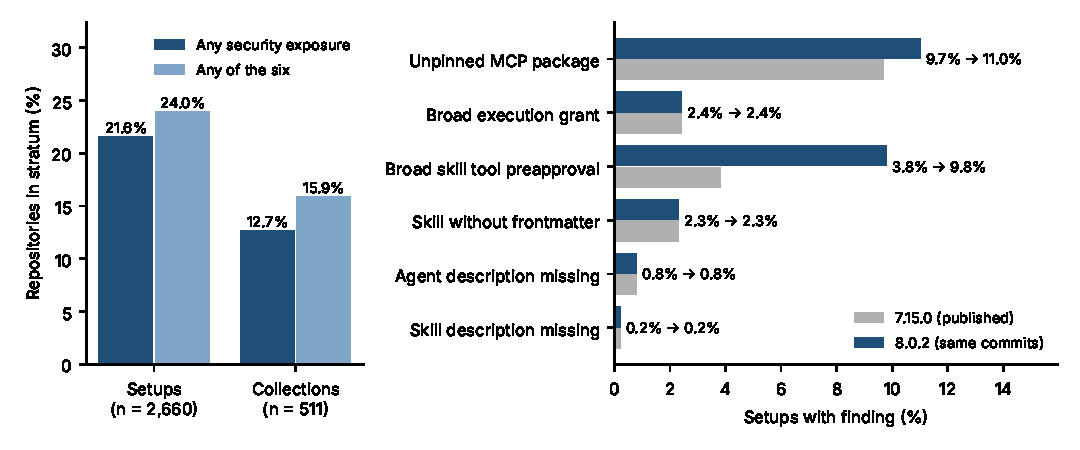
\includegraphics[width=\columnwidth]{../figures/results_v802.pdf}
\caption{Left: the union of security exposures and the union of the six categories under \vnew{}. Right: per-category setup proportions under \vold{} (published) and \vnew{} on the same commits.}
\label{fig:results}
\end{figure}

Table~\ref{tab:categories} and Figure~\ref{fig:results} summarize the six categories. \SOneSetups{} setups (\pct{\SOneSetupsPct}) declare an unpinned MCP package in live configuration; among the \DenSetupsWithMcp{} setups with MCP configuration, the proportion is \pct{\CondSOneofmcp}. \STwoSetups{} setups (\pct{\STwoSetupsPct}) carry a broad execution grant in settings, \pct{\CondSTwoofhooks} of the \DenSetupsWithHooks{} setups with a hooks or settings component. \SThreeSetups{} setups (\pct{\SThreeSetupsPct}) and \SThreeCols{} collections (\pct{\SThreeColsPct}) preapprove a shell, interpreter, or package runner in a skill; among setups that contain skills the proportion is \pct{\CondSThreeofskills}. The union of the three exposure categories covers \AnySSetups{} setups (\pct{\AnySSetupsPct}), against \AnySOldSetups{} (\pct{\AnySOldSetupsPct}) when the same policy is applied to the \vold{} records of the same bytes. Missing agent descriptions affect \QOneSetups{} setups (\pct{\QOneSetupsPct}; \pct{\CondQOneofagents} of setups with subagents). Skills without frontmatter occur in \POneSetups{} setups and \POneCols{} collections; a present block without a description in \PTwoSetups{} setups. The union of all six is \AnySixSetups{} setups (\pct{\AnySixSetupsPct}) and \AnySixCols{} collections (\pct{\AnySixColsPct}).

\textbf{Accounting.} Table~\ref{tab:ladder} fixes the rule set and applies five restrictions in order, for both instruments. The first iteration reported 678, 503, 488, and 475 setups for its four stages; its ``raw'' rows already included the finding-class split that is our third stage, and its last stage applied model-assisted inclusion decisions. Our class and semantic-correction stages reproduce its 503 and 488 exactly on the \vold{} records, and our mechanical final stage gives \LadderOldFinal{} setups (\pct{\LadderOldFinalPct}) against the published 475: path exclusions and the undetermined-wrapper rule reach the same union within four repositories, without a model. Under \vnew{} the ladder reads \LadderNewRawThirtyOne{}, \LadderNewRawSix{}, \LadderNewClass{}, \LadderNewNofind{}, and \LadderNewFinal{} setups; the semantic-correction row no longer changes the count because the instrument carries the correction. Because conditions overlap, the marginal reductions depend on order and are not independent effects.

\begin{table}[t]
\centering
\caption{Fixed-rule accounting for the setup union, both instruments on the pinned commits. Each row applies the stated restriction to the row above.}
\label{tab:ladder}
\small
\begin{tabular}{@{}lrrrr@{}}
\toprule
Analysis stage (setups, n = 2,660) & \multicolumn{2}{c}{7.15.0} & \multicolumn{2}{c}{8.0.2} \\
\midrule
Any of the 31 candidate rules fired & 769 & 28.9\% & 1064 & 40.0\% \\
Any of the six selected rules fired & 602 & 22.6\% & 954 & 35.9\% \\
Six rules, exposure or specification class only & 503 & 18.9\% & 656 & 24.7\% \\
Documented \texttt{find}/\texttt{watch} exception applied & 488 & 18.3\% & 656 & 24.7\% \\
Path exclusions and undetermined wrappers removed & 471 & 17.7\% & 639 & 24.0\% \\
\bottomrule
\end{tabular}

\end{table}

\subsection{Declaration-Level Denominator}
\label{sec:declarations}

\begin{table}[t]
\centering
\caption{Every MCP server declaration found in setups (Scan B), classified by transport and pin state independently of any rule. Package declarations are those run through a package runner or container image.}
\label{tab:declarations}
\small
\begin{tabular}{@{}lr@{}}
\toprule
MCP server declarations in setups & Count \\
\midrule
Declarations (files: 2,593) & 3,923 \\
\quad remote (URL) & 1,488 \\
\quad local command or script & 959 \\
\quad package runner (npx, uvx, pipx, bunx, docker) & 1,476 \\
\qquad pinned (exact version or digest) & 157 \\
\qquad floating tag (\texttt{@latest}, \texttt{:latest}) & 190 \\
\qquad no version & 1,129 \\
\bottomrule
\end{tabular}

\end{table}

A repository rate conflates repositories with one declaration and repositories with twenty, and it hides what the unflagged majority of MCP-bearing setups actually declare. Scan B therefore inventories every MCP server declaration in each tree, independently of the scanner's rule, and classifies it by transport and pin state (Table~\ref{tab:declarations}). Of \DeclTotal{} declarations in setups, \DeclRemote{} name a remote URL, \DeclLocal{} run a local command or script, and \DeclPackage{} (\pct{\DeclPctPackage}) run a package through a runner or a container image. Of the package declarations, \DeclPackagePinned{} pin an exact version or digest, \DeclPackageTag{} name a floating tag, and \DeclPackageUnpinned{} give no version at all; \pct{\DeclPctUnpinnedOrTag} of package declarations float. This is the number a pinning recommendation should be judged against: the unpinned form is the documented default in most server READMEs, and the declaration-level rate says how far the ecosystem has moved from it.

\subsection{RQ3: Persistence at the Current Default Branch}
\label{sec:persistence}

\begin{table}[t]
\centering
\caption{Persistence. Repositories flagged in Scan B (pinned commit) and their state in Scan C (default branch, five weeks later, same instrument). \emph{Resolved} means the repository rescanned clean for that category; \emph{gone} means it could not be fetched; \emph{new} means flagged at HEAD only.}
\label{tab:persistence}
\small
\begin{tabular}{@{}llrrrrr@{}}
\toprule
ID & Finding & At pin & Still & Resolved & Gone & New \\
\midrule
S1 & Unpinned MCP package declaration & 294 & 277 & 17 & 0 & 2 \\
S2 & Broad execution grant (settings) & 63 & 62 & 1 & 0 & 0 \\
S3 & Broad skill tool preapproval & 325 & 313 & 12 & 0 & 3 \\
Q1 & Agent description missing & 20 & 19 & 1 & 0 & 0 \\
P1 & Skill without frontmatter & 80 & 75 & 5 & 0 & 0 \\
P2 & Skill description missing & 6 & 2 & 4 & 0 & 0 \\
\bottomrule
\end{tabular}

\end{table}

Of the \NPinnedOk{} repositories rescanned at the pin, \NMovedHead{} (\pct{\PctMovedHead}) had a different default-branch head at scan time. \NHeadUnfetchable{} corpus repositories could not be fetched at HEAD, but \NGoneAfterPin{} of those had been fetchable at the pin: attrition between the September pin and the October scan is small, and almost every unfetchable repository was already gone when the pinned rescan ran. Table~\ref{tab:persistence} follows each category. \PersSOneResolvedAtHead{} of \PersSOneFlaggedAtPin{} unpinned-declaration repositories rescanned clean at HEAD (\pct{\PersSOneResolvedPctOfRescanned} of those rescanned), \PersSOneStillAtHead{} still carried the condition, and \PersSOneNewAtHead{} repositories acquired one. For broad settings grants, \PersSTwoResolvedAtHead{} of \PersSTwoFlaggedAtPin{} were resolved and \PersSTwoNewAtHead{} appeared; for skill preapproval, \PersSThreeResolvedAtHead{} of \PersSThreeFlaggedAtPin{} were resolved and \PersSThreeNewAtHead{} appeared. A resolved category does not mean a maintainer judged it a defect: a skill may have been deleted or rewritten for other reasons, and we did not read commit messages. The numbers nonetheless bound how much of the measured exposure is stable over the interval: more than half of the repositories changed, and the three exposure categories persisted in over ninety percent of the repositories that carried them, so they are not transient artifacts of a single snapshot.

\subsection{RQ4: Validation and What the First Iteration Missed}
\label{sec:validation}

\begin{table}[t]
\centering
\caption{Validation of the \vnew{} findings. Mechanical re-derivation per finding, and the first iteration's human verdicts joined to the \vnew{} repository-rule pairs. \emph{Agree} is agreement between the human verdict and the mechanical inclusion decision on rated pairs.}
\label{tab:validation}
\footnotesize
\IfFileExists{../data/v802/tex/tab_validation.tex}{\begin{tabular}{@{}lrrrrrr@{}}
\toprule
ID & Findings & Re-derived & Refuted & Unverif. & Rated pairs & Agree \\
\midrule
S1 & 1,038 & 1,038 & 0 & 0 & 268/307 & 98.5\% \\
S2 & 232 & 232 & 0 & 0 & 70/87 & 90.0\% \\
S3 & 4,602 & 4,602 & 0 & 0 & 118/436 & 96.6\% \\
Q1 & 158 & 157 & 1 & 0 & 23/23 & 78.3\% \\
P1 & 7,176 & 6,976 & 18 & 182 & 77/631 & 100.0\% \\
P2 & 69 & 69 & 0 & 0 & 4/6 & 100.0\% \\
\bottomrule
\end{tabular}
}{\textit{(audit pending)}}
\end{table}

\textbf{Mechanical agreement.} The audit re-derived \AuditFindings{} findings over \AuditRepos{} repositories (Table~\ref{tab:validation}); the frontmatter sub-checks account for most findings because one skill can carry several. Agreement is \pct{\AuditSOneAgree} for unpinned declarations, \pct{\AuditSTwoAgree} for settings grants, \pct{\AuditSThreeAgree} for skill preapproval, and above \pct{99} for the three format categories. Two details of how the audit reached those numbers belong in the record. Its first pass refuted 56 unpinned declarations that it could not see: they live in Codex TOML files, OpenCode configurations that write the command as one argument array, and plugin bundles' nested files, none of which the audit's reader parsed, and a declaration the audit cannot read is now reported as unverifiable rather than refuted. Its first pass also refuted 27 skill grants because the finding's message was truncated at the record boundary; the audit now reads the structured tool list the scanner records. The \AuditPOneUnverifiable{} unverifiable frontmatter findings name skills in discovery roots the audit's skill finder does not enumerate. Agreement of this kind measures consistency between two implementations of one specification; the \texttt{find} case shows that it can be complete and wrong at the same time, and the two audit corrections show that a refutation can be the audit's gap rather than the scanner's.

\textbf{Human verdicts.} The first iteration's \HumanTotalVerdicts{} human verdicts cover \HumanSOneWithHumanVerdict{} of the \HumanSOnePairsNew{} \vnew{} repository-rule pairs in S1 and agree with the mechanical inclusion decision in \pct{\HumanSOneAgreePct} of them; the \HumanSOneHumanYesButExcluded{} disagreements are declarations under template or fixture paths that the human called defects and the path rule reports apart. For S2, \HumanSTwoWithHumanVerdict{} of \HumanSTwoPairsNew{} pairs are rated with \pct{\HumanSTwoAgreePct} agreement; the \HumanSTwoHumanYesButExcluded{} disagreements are five bare \texttt{Edit} or \texttt{Write} grants and two stripped-wrapper grants (\texttt{timeout}, \texttt{xargs}) that the human counted as exposures and this policy reports in their own classes, a documented difference of reading rather than an error on either side. For Q1, \HumanQOneWithHumanVerdict{} of \HumanQOnePairsNew{} pairs are rated with \pct{\HumanQOneAgreePct} agreement, the lowest of the six: \HumanQOneHumanYesButExcluded{} files in a root-level \texttt{agents/} directory that the human read as subagent definitions and the policy excludes, and \HumanQOneHumanNoButIncluded{} the policy includes and the human cleared; the category is small enough that these five pairs are listed in the artifact. For S3, \HumanSThreeWithHumanVerdict{} of \HumanSThreePairsNew{} pairs are rated with \pct{\HumanSThreeAgreePct} agreement (\HumanSThreeHumanNoButIncluded{} bare \texttt{Bash} grants the human cleared, in skills written for clients that do not read the field, and \HumanSThreeHumanYesButExcluded{} scoped grant the human counted), and \HumanSThreeNewPairsWithoutVerdict{} pairs are new under \vnew{} and have no human verdict at all. We report this gap rather than fill it with a model: the new pairs are the string-form grants the first instrument missed, and the appropriate check is a fresh human reading with a second rater, which is future work.

\textbf{What the first iteration's validation missed.} Its mechanical audit reported 97--100\% agreement per rule; its human review agreed with the pipeline on 93.3\% of pairs ($\kappa=0.76$) overall and on 70.7\% ($\kappa=0.23$) of the 157 model-adjudicated pairs. Neither number could have revealed the parser gap, because every check consumed the scanner's output. The model adjudication moved the headline from 18.3\% to 17.9\% at near-chance agreement with the human on the pairs it decided, which is why this iteration drops it from the headline and keeps it only as a historical comparison. Six repositories flagged by an exploratory credential-to-network graph rule were read by hand in the first iteration and none established the claimed exfiltration path; that result stands and is not re-measured here.

\section{Implications}

\textbf{For maintainers and publishers.} The declaration-level table (Table~\ref{tab:declarations}) is the actionable one: \pct{\DeclPctUnpinnedOrTag} of package-runner declarations float. Pinning the version or image digest makes the selected code explicit; controlling transitive dependencies additionally needs a lockfile or resolved manifest. For execution preapproval, the question is whether the breadth of the grant matches the task; \texttt{Bash(python:*)} covers any Python program, and a skill that lists \texttt{Bash} preapproves every shell command for its turn. Publishers can check skill frontmatter against the specification before distribution, since \vnew{}'s type checks found deviations in \pct{\PThreeSetupsPct} of setups that a permissive client loads without complaint.

\textbf{For analyzer authors.} Two of this study's own defects were invisible to cross-implementation agreement and to a human reading of the scanner's output. The remedies are specific. First, version the client semantics: each permission predicate should carry the documentation it was read from and a test for every documented exception, so that a changed client behavior is a failing test rather than a paper correction. Second, run an instrument-change experiment on every release that touches a measured rule: the same pinned corpus, the previous and the new version, and an attributed table of lost and gained repositories. The \vold{} to \vnew{} table (Table~\ref{tab:instrument}) took one scan and found a recall defect that a year of output-side validation had not.

\textbf{For measurement studies.} Report fixed-rule accounting (Table~\ref{tab:ladder}) alongside the headline, report repository and declaration denominators, and keep model adjudication out of headline numbers unless its agreement with human judgment on the pairs it decides is itself measured and adequate. Persistence scans are cheap and separate ecosystem change from instrument change, which a single snapshot cannot do.

\section{Threats to Validity}

\textbf{Construct validity.} We measure declarations and field omissions. A security exposure is not an exploit, a broad grant need not be unwanted, and a specification deviation need not cause a failure. We have not measured users' expectations, workspace trust, activation, sandboxing, or attacker control. Documented semantics differ by client and version; our correction addresses one documented exception and one documented wrapper class, and the remaining grant patterns have not been tested against a running client. The rule vocabulary omits some code-executing build tools and version-control grants. The MCP declaration classifier was written for the npx, uvx/pipx, and docker argument grammars and may misclassify unusual invocations; its code is in the artifact.

\textbf{Internal validity.} The mechanical inclusion policy is ours, and its path patterns encode a judgment that fixture and template declarations are distributed examples rather than live configuration; a reader who disagrees can read the class-stage row of Table~\ref{tab:ladder} instead. The audit and the scanner share a rule vocabulary by design; the documentation check, not their agreement, is the defense against a shared error, and it was performed by the authors.

\textbf{Label validity.} The human verdicts were recorded by one author on \vold{} pairs; their agreement with the mechanical policy is not inter-rater reliability, and the S3 pairs gained under \vnew{} have no human verdict. Recall remains unmeasured: the parser gap was found by an instrument change, not by a recall study, and other gaps of the same kind may exist.

\textbf{External validity.} Discovery favors visible, advertised configurations. Proportions are not weighted by users, downloads, or installations. Heuristic deduplication does not remove every shared template, and fork metadata was not used. Private configurations may differ. Repositories that disappeared between the pin and the HEAD scan may differ systematically from those that remained.

\textbf{Reproducibility.} Input commits, scanner versions, scan timestamps, and output records are pinned and released. Scan B reproduces the instrument comparison exactly; Scan C depends on the state of GitHub on October 10, 2026, and a later scan will differ.

\section{Conclusion}

Rescanning a fixed corpus with a corrected instrument changed the measured prevalence of agent-configuration exposures in both directions and exposed a parser gap that had hidden a large share of one category. Under the corrected scanner and a mechanical, re-derivable inclusion policy, \pct{\AnySSetupsPct} of \NSetups{} assembled setups carry an unpinned MCP package or a broad execution preapproval, \pct{\DeclPctUnpinnedOrTag} of package-runner declarations float, and a five-week persistence scan shows most flagged conditions still present. The methodological result is the more durable one: cross-implementation agreement and model adjudication did not detect either instrument defect, a documentation check and an instrument-change experiment did, and configuration-scan studies of agent supply chains should treat both as part of the measurement.

\section*{Data Availability}
The corpus list with pinned commits, the three scan outputs, the audit records, the human verdicts, the inclusion policy, the reanalysis and figure scripts, and the scanner source at both versions are in the anonymized artifact (URL withheld for double-blind review). The artifact stores URLs, commits, findings, and evidence lines; no third-party repository content. One credential-like literal is redacted from scanner evidence.

\section*{Use of AI Assistance}
Language models assisted with prose revision and with the reanalysis and figure code. They produced no corpus observations, no human verdicts, and no inclusion decisions in this iteration.

\balance
\bibliographystyle{IEEEtran}
\bibliography{refs}

\end{document}
